\section{Incremental Synchronization of Shapes}
%\td{\emph{Our} simple impl., \emph{our} patch formalism, \emph{our} dispatch, \etc}

\td{@Fabien:~imho, your definitions should describe what is depicted in \Cref{fig:concepts}. This is the basis to then describe \Cref{fig:prism} which builds upon these concepts to detail our approach. Could be two subsections.}

The cornerstone artifact defining a DSL in any LV is its abstract syntax.
The way abstract syntax is expressed differs drastically from one LV to another: GEMOC~\cite{bousse2016execution} and Xtext~\cite{bettini2016implementing}---under the hood---use Ecore metamodels~\cite{steinberg2008emf}; MPS\footnote{\url{https://www.jetbrains.com/mps/}} uses \emph{concepts}; Rascal~\cite{klint2010easy} uses Algebraic Data Types (ADT); \etc.
Language embedding techniques, on the other hand, use the constructs of an host language to materialize the abstractions of a DSL in the host language itself (\eg~a set of Java classes).
Concrete models are then built as instances of the corresponding abstract syntax formalism:~Ecore models, ADT values, Java ASTs, \etc.
The tools defined within a particular LV (\eg~an interpreter in Rascal, an editor in EMF) manipulate models in the appropriate formalism (respectively, ADT values and Ecore models).
Thus, bridging various LV requires to:
\begin{enumerate}
	\item Synchronize the various in-memory representations of the same model;
	\item Allow every LV to maintain the extra information it needs to properly work (layout information in graphical and textual editors, runtime state, AST context, \etc);
	\item From 1. and 2., it follows that the synchronization must be incremental.
\end{enumerate}

\Cref{fig:prism} depicts our approach, \prism.

\begin{figure}
	\centering
	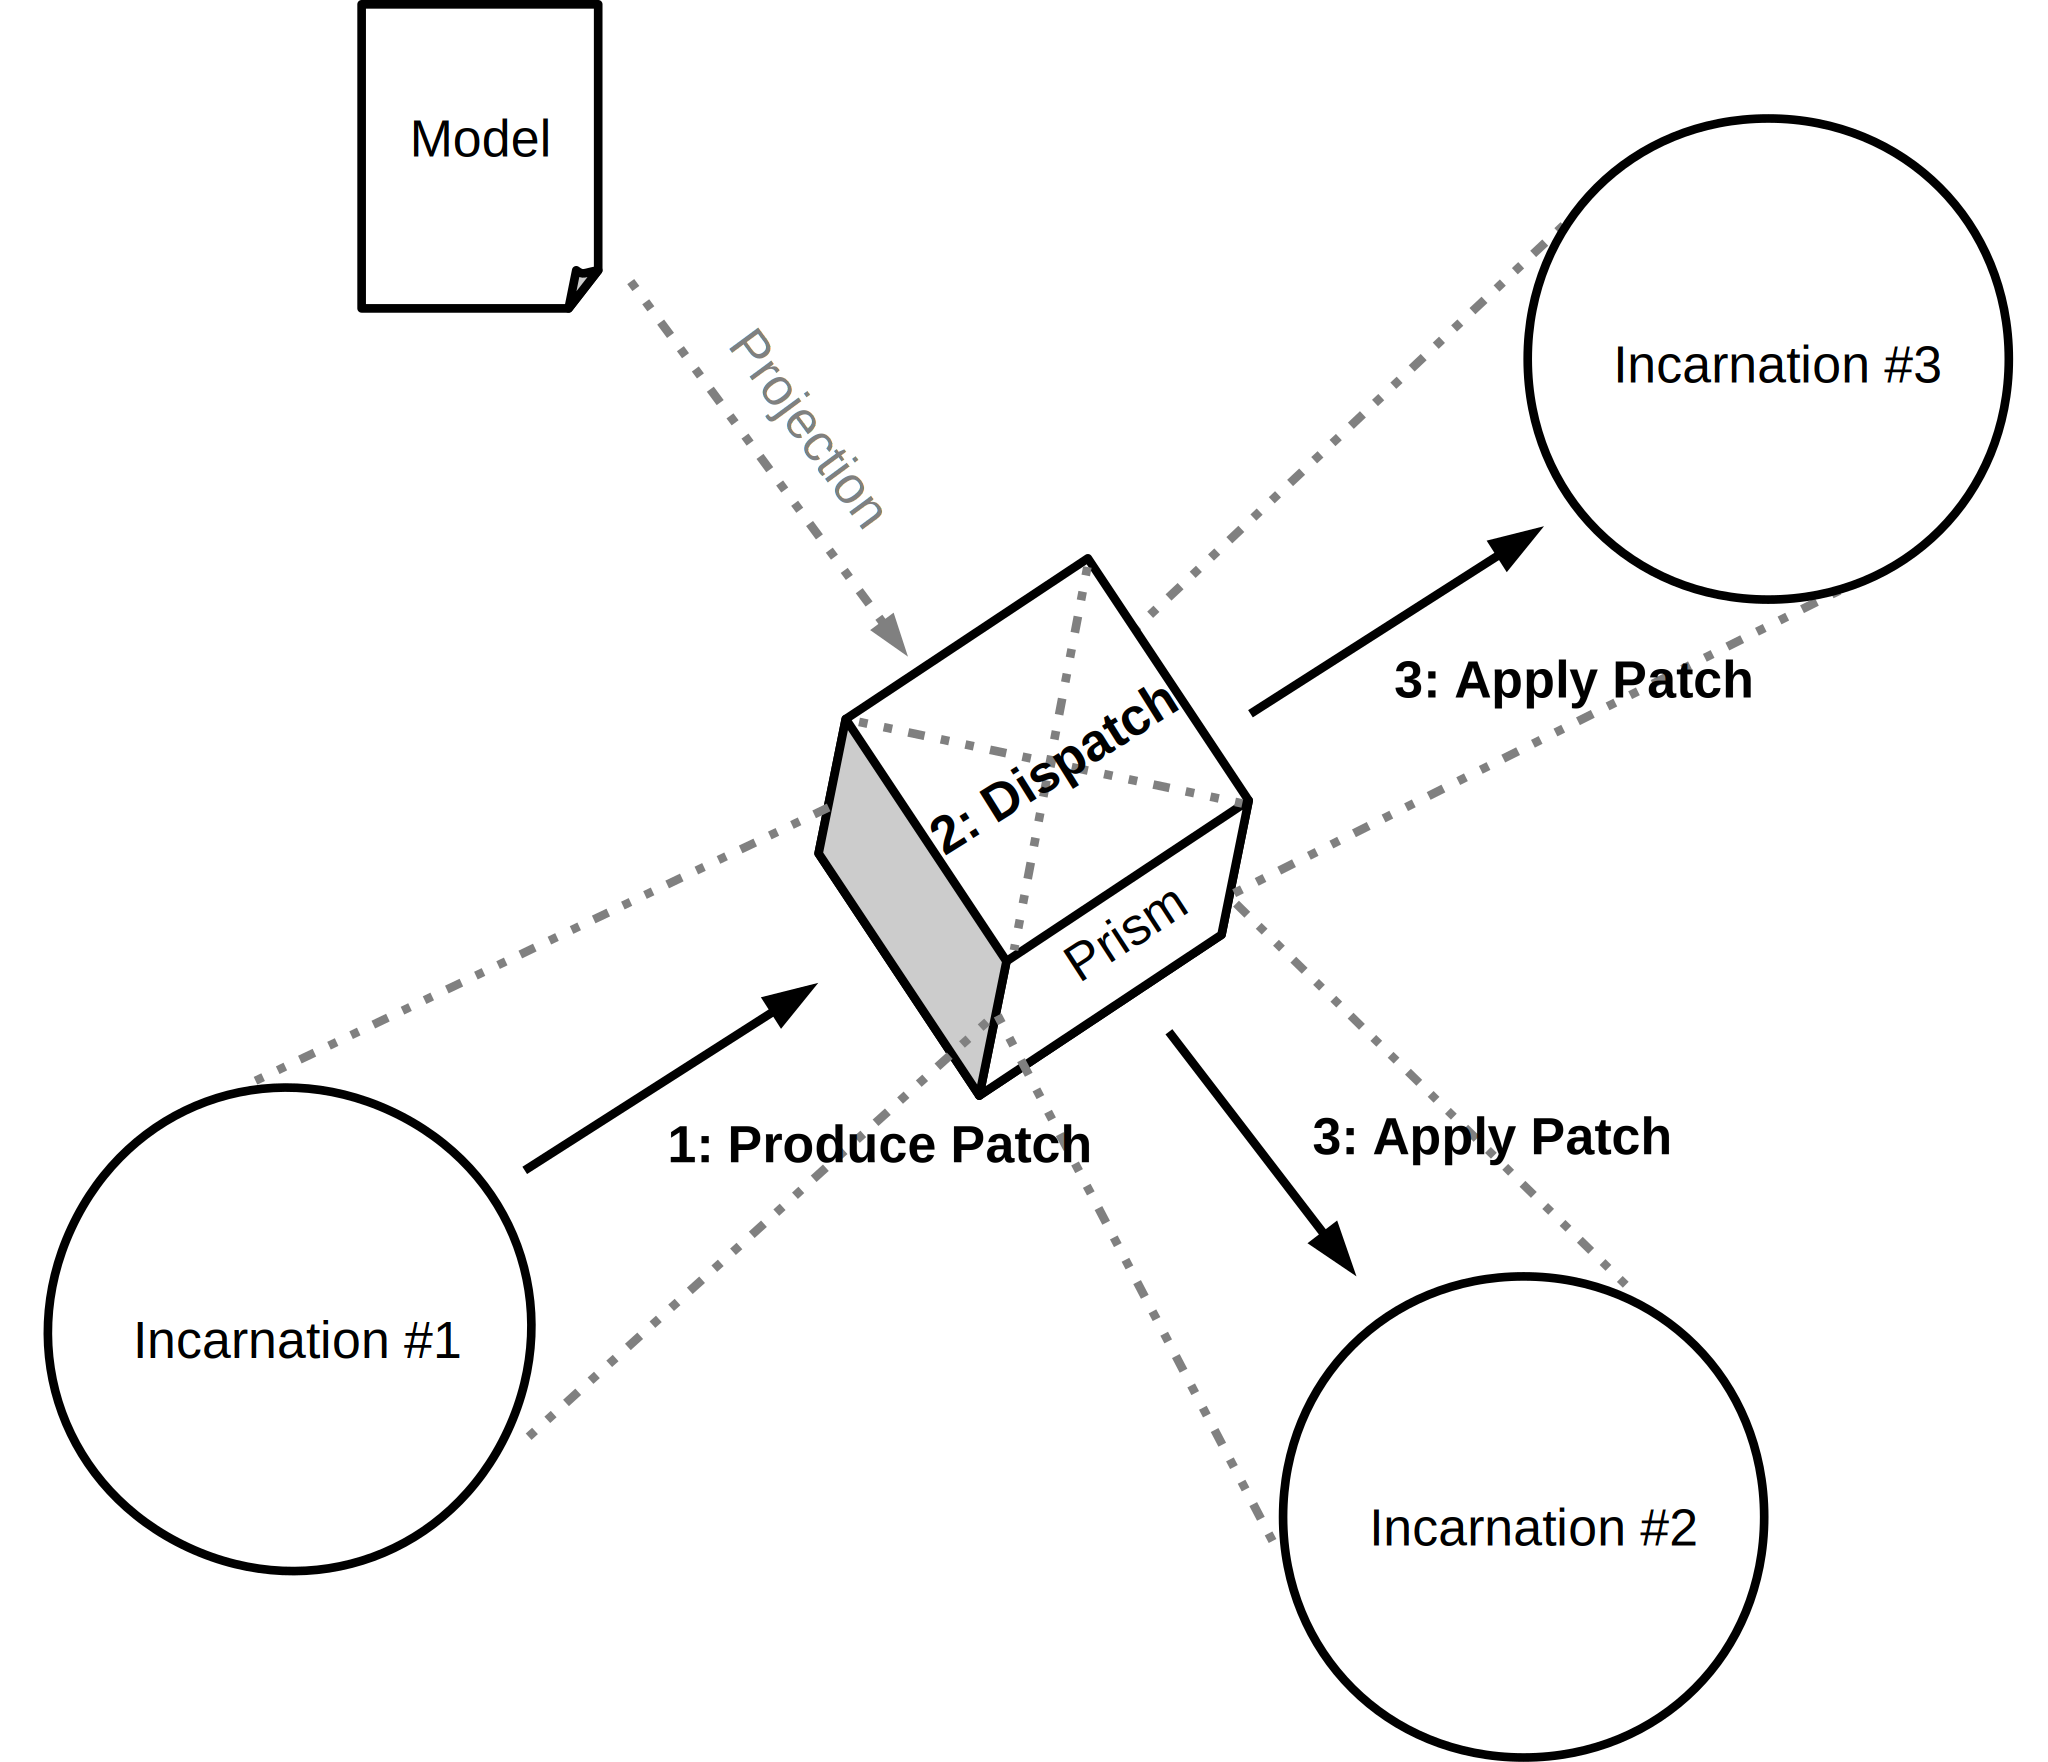
\includegraphics[width=.6\columnwidth]{figures/prism}
	\caption{A model projected in different LVs}
	\label{fig:prism}
\end{figure}

\begin{figure}
	\centering
	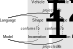
\includegraphics[width=.8\columnwidth]{figures/concepts}
	\caption{Languages (resp.~models) are projected as shapes (resp.~incarnations) in LVs. Just as models conform to languages, incarnations conform to shapes.\\NB: \emph{projectedAs $\Rightarrow$ realizedBy} or something else?}
	\label{fig:concepts}
\end{figure}

A naive way to bridge different LV would be to define bidirectional transformations between the abstract syntax formalisms of every pair $\langle LV, LV' \rangle$.
Doing so however would break \emph{incrementality}, \ie~it would not be possible to maintain the extra information every TS holds, such as layout in a editor or runtime data when running models.
In our approach, instead, every change occuring on one side is shipped to all the other sides.
The latter then decide which parts of the changes they want to take into account.
An outline, for instance, would probably ignore most of the changes and focus on some of them. Argh.

Bridging multiple TS thus requires to ``align'' in some ways the representation of the AS of a language in these different TS.
As an illustration, the EMF and the Rascal LWB expose fundamental differences:~object-oriented vs. functional, graphs vs. trees, mutable ASG vs. immutable ASTs, cross-references vs. symbolic names, \etc.
However, it is neither possible nor desirable to establish a common formalism upon which various TS would agree:~mapping those is out of reach.

The key underlying idea of our approach is to provide the capability, at any time, to ``project'' a given model in any of its shapes and to synchronize those shapes whenever one of them is updated.
We enable the projection of a given model as an ADT value, to be manipulated in the Rascal TS, or as an Ecore model, to be manipulated in the EMF TS.

Instead, our approach keeps the TS fully independent and builds a communication bus between them.
Both representations of the same model in various TS are kept in memory to allow online synchronization of the same models manipulated by different stakeholders in different shapes.
When a changes occurs on either side, this side is responsible for generating a \emph{patch} (aka. \de or edit script~\cite{rozen2017towards}), that stores the changes on the model that have been realized on this side.
The communication bus then ships this patch to all the other sides.
Every side interprets the patch in its own way to keep the representation synchronized.
On the EMF side, for instance, the patch is interpreted as a set of changes that impact an Ecore model, while on the Rascal side it is interpreted as a set of changes that impact a value conforming to the ADT defining the AS of the language.

It is important to note that each TS may want to preserve certain information across the patches that are specific to the TS.
A textual editor in Rascal, for instance, needs to keep some of the parsing information to maintain layout whenever patches are applied.
So it should be possible to apply the patch while maintaining the extra information specific to a given TS.

Automatically generating language implementations in different TS is beyond the scope of this paper.\footnote{Indeed, this would actually require to build some kind of BX between all AS formalisms; so, nope!} Instead, given various shapes of a language, implemented by hand, we provide the means to automatically synchronize the projections of a model.

\begin{lstlisting}[label=lst:delta-adt, caption={CRUD-like \ds structure definition in Rascal}, language=Rascal]
@doc{A patch consists of a sequence of edits}
alias Patch = tuple[Id root, Edits edits];

@doc{Edits are operations attached to object identities}
alias Edits = lrel[Id obj, Edit edit];

data Edit
  = put(str field, value val)
  | unset(str field)
  | ins(str field, int pos, value val)
  | del(str field, int pos)
  | create(str class) 
  | destroy();
\end{lstlisting}

It is important to note that ``projections'' have no relation whatsoever with projectional editing.
A projection denotes the incarnation of a model in a particular shape of a language.
In \Cref{fig:motivating-fsm}, the lower part depicts three projections of the same \texttt{Button} state machine model in three shapes of the FSM language.
We use the term ``language'' to refer to the specification of a language independently from its realization in a given TS.
A concrete implementation of a language is a ``shape''.
An instance of a shape, \ie~a particular model in a particular TS, is a ``projection'' of a ``virtual'' model.
Metamorphic synchronization refers to the ability to synchronize the projections of a given model for every shapes of a language.

\begin{definition}
A projection of model is a relation between a conceptual model and its different incarnations in the LVs.
All of theses incarnations represent the same model but in different formalisms and technologies.
Incarnations have to be synchronized, i.e., any change on an incarnation is a change on the conceptual model and thus other incarnations have to apply the same change.
\end{definition}

\begin{definition}
An incarnation is in the context of a model projection what is representing the model in a given LV.
\end{definition}

\begin{definition}
A prism in the context of a model projection is the mechanism that allows the different incarnations of the model to be in equivalent state and to synchronize.
\end{definition}

\begin{definition}
A shape is a projection of a language in a particular LV.
It is equivalent to a language implementation in a LV.
Therefore if a model is conform to the language, all its incarnations in this LV are conform to the shape.
\end{definition}
